\subsection{Fixed Income Risk}

\begin{remark} \hlt{Sources of Return in Fixed-Rate Bond}
\begin{enumerate}[label=\roman*.]
\setlength{\itemsep}{0pt}
\item Coupon and principal payments
\item Interest earned on coupon payments that are reinvested over holding period
\item Capital gain or loss if bond is sold before maturity
\end{enumerate}
\end{remark}

\begin{remark} \hlt{Performance of Return}\\
Assuming no credit risk, and the interest rate earned on reinvested coupon payments is the same as prevailing YTM on the bond, there are five key results:
\begin{enumerate}[label=\roman*.]
\setlength{\itemsep}{0pt}
\item Unchanged YTM, bond held to maturity: investor will earn annualised rate of return equal to YTM of the bond when purchased
\item Unchanged YTM, bond sold before maturity: investor will earn YTM of the bond
\item Changed YTM, bond held to maturity: if rates increase after the bond is purchased before first coupon date, holding a bond to maturity will earn rate of return greater than YTM at purchase
\item Changed YTM, bond sold before maturity in short period: if rates increases after bond is purchased before first coupon date, investor will earn lower than YTM at purchase
\item Changed YTM, bond sold before maturity in long period: if rates decreases after bond is purchased before first coupon date, investor will earn lower than YTM at purchase
\end{enumerate}
\end{remark}

\begin{definition} \hlt{Price Risk}\\
The uncertainty on bond's price due to uncertainty about prevailing market YTM at time of sale
\end{definition}

\begin{definition} \hlt{Reinvestment Risk}\\
The uncertainty about total coupon payments and reinvestment income on these payments due to uncertainty about future reinvestment rates.
\end{definition}

\begin{remark} \hlt{Price Risk vs Reinvestment Risk}
\begin{enumerate}[label=\roman*.]
\setlength{\itemsep}{0pt}
\item Short investment time horizon: price risk > reinvestment risk
\item Long investment time horizon: price risk < reinvestment risk
\end{enumerate}
Premium bond is more dependent on reinvestment income than par bond.\\
Zero-coupon bonds has no reinvestment risk if held to maturity as there is no periodic cash flow to be reinvested.
\end{remark}

\subsubsection{Yield-Based Duration and Convexity Measures}

\begin{definition} \hlt{Bond Duration}\\
Measures sensitivity of bond’s full price to changes in bond’s own yield, or to changes in benchmark rate.\\
Represents approximate amount of time a bond to be held for market discount rate to be realised.
\end{definition}

\begin{definition} \hlt{Yield Duration}\\
Sensitivity of bond price to its own YTM.\\
May be Macaulay, Modified, Money, Price Value of a Basis Point (PVBP)
\end{definition}

\begin{definition} \hlt{Curve Duration}\\
Sensitivity of price to benchmark yield, as measured by effective duration.\\
Change in benchmark yield not equal same change in bonds YTM, to be measured based on par curve.
\end{definition}

\begin{definition} \hlt{Portfolio Duration}\\
Weighted average of duration of individual bonds in portfolio.\\
Can be used for bonds with embedded options. However, using cash flow yield is theoretical correct.
\end{definition}

\begin{definition} \hlt{Macaulay Duration Long Form}
\begin{equation}
\text{MacDur} = \frac{\sum\limits_{n=1}^N \frac{(n - t/T) \times PMT}{(1+r)^{n - t/T}} + \frac{(N - t/T) \times FV}{(1+r)^{N - t/T}}}{\sum\limits_{n=1}^N \frac{PMT}{(1+r)^{n - t/T}} + \frac{FV}{(1+r)^{N - t/T}}} \nonumber
\end{equation}
where $t$ is days from last coupon payment to settlement date, $T$ is number of days in coupon period, $PMT$ is coupon payment per period, $FV$ is future value paid at maturity or par value of bond, $r$ is YTM or market discount rate per period, $N$ is number of evenly spaced periods to maturity as of beginning of current period.\\
Note that the denominator is the full price of bond including accrued interest.
\begin{equation}
PV^{\text{Full}} = \sum\limits_{n=1}^N \frac{PMT}{(1+r)^{n - t/T}} + \frac{FV}{(1+r)^{N - t/T}} \nonumber
\end{equation}
\end{definition}

\begin{definition} \hlt{Macaulay Duration Closed Form}
\begin{equation}
\text{MacDur} = \left\{\frac{1+r}{r} - \frac{1+r+[N \times (c-r)]}{c \times [(1+r)^N - 1] + r} \right\} - \frac{t}{T} \nonumber
\end{equation}
where $c$ is coupon rate per period.
\end{definition}

\begin{definition} \hlt{Annualised Macaulay Duration}
\begin{equation}
\text{AnnMacDur} = \frac{\text{MacDur}}{\text{Number of coupon payments in a year}} \nonumber
\end{equation}
\end{definition}

\begin{flushleft}
\begin{tabularx}{\textwidth}{X|X|X}
\hline
\rowcolor{gray!30}
Scenario & Dominant Risk & Source of Interest Rate Risk \\
\hline
Investment Horizon $>$ MacDur & Reinvestment risk & Falling interest rates \\
\hline
Investment Horizon $=$ MacDur & Equal risk & $-$ \\
\hline
Investment Horizon $<$ MacDur & Price risk & Rising interest rates \\
\hline
\end{tabularx}
\end{flushleft}

\begin{figure}[H]
\centering
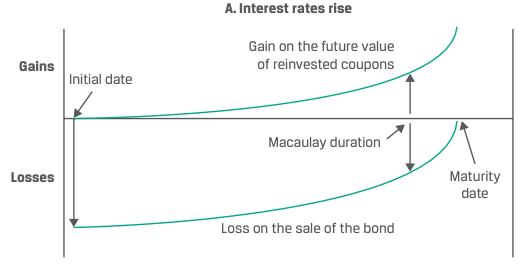
\includegraphics[scale=0.45]{/fi/macdurirrise}\hfill
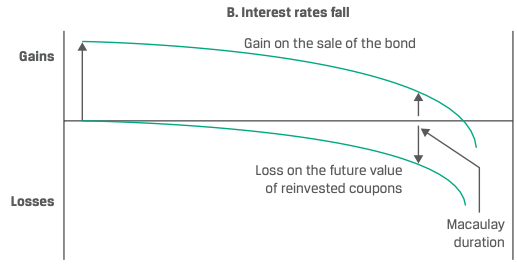
\includegraphics[scale=0.45]{/fi/macdurirdrop}
\caption{Interest rate effects on Macaulay Duration}
\end{figure}

\begin{remark} \hlt{Interpretation of Macaulay Duration}\\
Weighted average of time to receipt of bond’s promised payments, where the weights are shares of full price that correspond to each of the bond’s promised future payments
\end{remark}

\begin{method} \hlt{Computing Macaulay Duration}
\begin{enumerate}[label=\roman*.]
\setlength{\itemsep}{0pt}
\item Calculate PV of each payment for each period
\item Calculate weight of each payment as percentage of total PV
\item Take the weighted of each payment, multiply by $(i-t/T)$
\item Sum up the results from above step to get MacDur.
\end{enumerate}
\end{method}

\begin{definition} \hlt{Modified Duration}\\
Provides an estimate of the percentage price change for a bond given a change in YTM (linear estimate).
\begin{equation}
\text{ModDur} = \frac{\text{MacDur}}{1+r} \nonumber
\end{equation}
Annualised modified duration may be computed by dividing by the number of coupon periods per year.
\begin{equation}
\text{AnnModDur} = \frac{\text{ModDur}}{\text{Number of coupon payments in a year}} \nonumber = \frac{\text{AnnMacDur}}{1+r} \nonumber
\end{equation}
\end{definition}

\begin{remark} \hlt{Annualised Modified Duration and Full Bond Price Relationship}
\begin{equation}
\%\Delta PV^{\text{Full}} \approx - \text{AnnModDur} \times \Delta \text{Annualised Yield} \nonumber
\end{equation}
If interest rate increase, price of bond decrease, and yield $>0$, thus $PV^{\text{Full}}$ decrease.
\end{remark}

\begin{remark} \hlt{Approximate Modified Duration}\\
If Macaulay Duration is not known, Modified Duration may be approximated.
\begin{align}
\text{AnnModDur} &\approx \frac{(PV_{-}) - (PV_{+})}{2 \times (\Delta \text{Yield}) \times PV_0} \nonumber \\
\text{AnnMacDur} &\approx \text{AnnModDur} \times (1+r) \nonumber
\end{align}
for a small $\Delta$Yield.
\end{remark}

\begin{figure}[H]
\centering
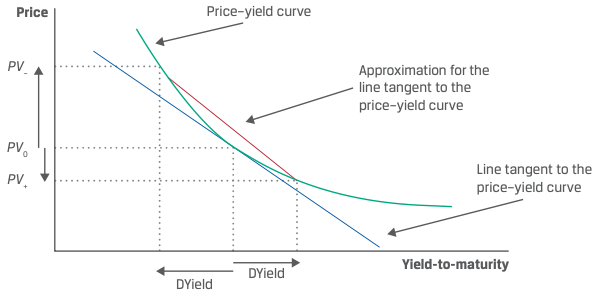
\includegraphics[scale=0.55]{/fi/moddurapprox}
\caption{Approximating modified duration}
\end{figure}

\begin{definition} \hlt{Money Duration}\\
A measure of the price change in currency units. The money duration can be stated per $100$ of par value or in terms of the actual position size.
\begin{align}
\text{MoneyDur} &= \text{AnnModDur} \times PV^{\text{Full}} \nonumber \\
\%\Delta PV^{\text{Full}} &\approx - \text{MoneyDur} \times \Delta \text{Yield} \nonumber
\end{align}
\end{definition}

\begin{definition} \hlt{Price Value of a Basis Point (PVBP)}\\
An estimate of the change in the full price of a bond given $1$ bp change in its yield-to-maturity.
\begin{equation}
\text{PVBP} = \frac{(PV_{-}) - (PV_{+})}{2} \nonumber
\end{equation}
\end{definition}

\begin{flushleft}
Summary of Yield-Based Duration Measures
\begin{tabularx}{\textwidth}{p{5em}|X|X}
\hline
\rowcolor{gray!30}
Measure & Calculation & Use \\
\hline
MacDur & Average time to receipt of promised cash flows, weighted by shares of the full price corresponding to each promised future cash flow & Holding period that would balance reinvestment and price risks\\
\hline
ModDur & First derivative of price with respect to yield. MacDur divided by $1 +$ yield per period & Estimate percentage price change for a bond given a change in its yield-to-maturity \\
\hline
MoneyDur & Modified duration multiplied by full price of bond or bond position & Estimate price change in bond investment for a given yield change \\
\hline
PVBP & Difference in price of a $1$ bp yield decrease and a $1$ bp yield increase, divided by $2$ & Estimate of the change in the bond price given a $1$ bp change in the yield-to-maturity \\
\hline
\end{tabularx}
\end{flushleft}

\begin{remark} Duration of Zero-Coupon Bond\\
As zero-coupon bonds have a single payments, face value at maturity, present weighted-average time to receipt of cash flows is same as time-to-maturity as that single cash flow has a present value weight of $1$.\\
Macaulay duration of a zero-coupon bond is its time-to-maturity, modified duration is time-to-maturity divided by $1$ plus yield.
\end{remark}

\begin{remark} Duration of Perpetual Bond\\
Bond does not mature, so there is no face or maturity value received at time $T$.\\
Non-callable perpetuities have Macaulay duration of $(1+r)/r$.
\end{remark}

\begin{remark} Duration of Floating-Rate Notes\\
Interest rate risk arises only between reset dates, as at the next reset date, coupon payments will adjust to the new MRR. Hence, the Macaulay duration for a floating-rate note or bond is simply the fraction of a period remaining until the next reset date, $(T-t)/T$.
\end{remark}

\begin{flushleft}
Properties of Yield Duration Statistics
\begin{tabularx}{\textwidth}{p{20em}|X}
\hline
\rowcolor{gray!30}
Increase in Feature & Effect on Duration (Interest Rate Risk) \\
\hline
Coupon rate $c$ & $\downarrow$ (inverse relationship) \\
\hline
Yield-to-maturity $r$ & $\downarrow$ (inverse relationship) \\
\hline
Time-to-maturity $T$ & $\uparrow$ (direct relationship) \\
\hline
Fraction of current coupon period elapsed $t/T$ & $\downarrow$ (inverse relationship) \\
\hline
\end{tabularx}
\end{flushleft}

\begin{figure}[H]
\centering
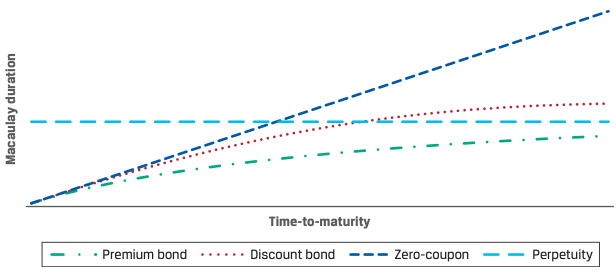
\includegraphics[scale=0.5]{/fi/macdurprop}
\caption{Properties of Macaulay Duration}
\end{figure}

\begin{definition} \hlt{Convexity}\\
Measures non-linear effect of yield changes on price for an option-free fixed-rate bond.\\
Fixed-rate bond will have greater convexity from:
\begin{enumerate}[label=\roman*.]
\setlength{\itemsep}{0pt}
\item longer time-to-maturity
\item lower coupon rate
\item lower yield-to-maturity
\item greater dispersion (degree to which payments are spread out over time)
\end{enumerate}
\end{definition}

\begin{figure}[H]
\centering
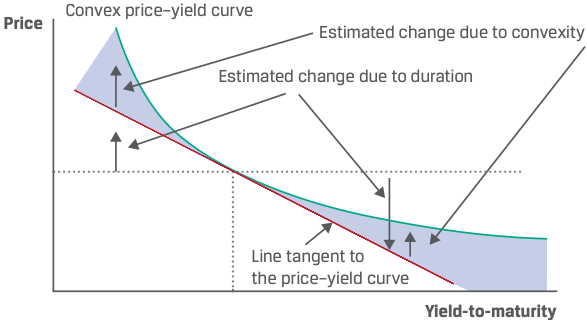
\includegraphics[scale=0.45]{/fi/convexity}
\caption{Convexity of an Option-Free Fixed-Rate Bond}
\end{figure}

\begin{remark} \hlt{Convexity Adjustment}
\begin{align}
\% \Delta PV^{\text{Full}} &\approx (-\text{AnnModDur} \times \Delta \text{Yield}) + \left[ \frac{1}{2} \times \text{AnnConvexity} \times (\Delta \text{Yield})^2 \right] \nonumber \\
\% \Delta PV^{\text{Full}} &\approx (-\text{MoneyDur} \times \Delta \text{Yield}) + \left[ \frac{1}{2} \times \text{MoneyConvexity} \times (\Delta \text{Yield})^2 \right] \nonumber
\end{align}
\end{remark}

\begin{flushleft}
Impact of changes in rates on duration and convexity
\begin{tabularx}{\textwidth}{p{10em}|X|X}
\hline
\rowcolor{gray!30}
Change in Rates & Impact on Duration & Impact on Convexity \\
\hline
$\Delta$BP $+$ & Negative & Positive \\
\hline
$\Delta$BP $-$ & Positive & Positive \\
\hline
\end{tabularx}
\end{flushleft}

\begin{definition} \hlt{Approximate Convexity}\\
Useful for bonds with uncertain cash flows, such as those with contingency features and default risk.
\begin{equation}
\text{ApproxConv} = \frac{(PV_{-}) + (PV_{+}) - [2 \times (PV_0)]}{(\Delta \text{Yield})^2 \times (PV_0)} \nonumber
\end{equation}
\end{definition}

\begin{figure}[H]
\centering
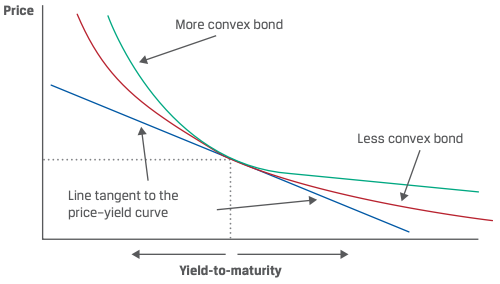
\includegraphics[scale=0.5]{/fi/convonoptfreebond}
\caption{Positive attributes of bond convexity on option-free bond}
\end{figure}

\begin{definition} \hlt{Exact Convexity}
\begin{equation}
\text{ExactConv} - \frac{[N - (t/T)] \times [N+1-(t/T)]}{(1+r)^2} \nonumber
\end{equation}
where $t/T$ is fraction of period that has passed, $r$ is YTM per period.
\end{definition}

\begin{remark} \hlt{Impact of Change in YTM on Convexity}\\
For two bonds with same price, YTM, and modified duration:\\
If YTM $\downarrow$, then the more convex bond will $\uparrow$ more in price.\\
If YTM $\uparrow$, then the more convex bond will $\downarrow$ less in price.\\
Hence, the more convex bond outperforms the less convex bond.\\
However, the more convex bond will have higher price, and lower YTM, hence investor have to pay for it.
\end{remark}

\begin{definition} \hlt{Weighted Average Time to Receipt of Aggregate Cash Flows}\\
Difficult in practice, as cash flow yield us not commonly calculated for bond portfolios.\\
Amount and timing of future cash payments are uncertain for bonds with embedded options or FRNs.\\
$\Delta$ cash flow yield is not the same as $\Delta$ YTM on individual bonds.\\
Interest rate risk is not usually expressed as $\Delta$ cash flow yield.
\end{definition}

\begin{definition} \hlt{Weighted Average Individual Bond Durations}\\
Easily used as measure of interest rate risk, i.e., $100$ bps rise in YTM, then estimated drop in portfolio is the average modified duration (AvgModDur).\\
Assumes parallel shift in yield curve. In reality, parallel shifts are rare.
\begin{align}
\text{AvgModDur} &= \sum\limits_{i=1}^N \text{ModDur}_i \left( \frac{\text{Bond}_{i, \text{Market Value}}}{\text{Portfolio Market Value}} \right) \nonumber \\
\text{ModDur}_i &= \frac{\text{AnnMacDur}_i}{1 + \frac{YTM_i}{m}} \nonumber
\end{align}
where $m$ is the periodicity.
\end{definition}

\subsubsection{Curve-Based and Empirical Duration and Convexity Measures}

\begin{definition} \hlt{Effective Duration}\\
Sensitivity of the bond’s price to a parallel change in a benchmark yield curve.
\begin{equation}
\text{EffDur} = \frac{(PV_{-}) - (PV_{+})}{2 \times \Delta \text{Curve} \times PV_0} \nonumber
\end{equation}
\end{definition}

\begin{definition} \hlt{Effective Convexity}
\begin{equation}
\text{EffConv} = \frac{(PV_{-}) + (PV_{+}) - [2 \times (PV_0)]}{(\Delta \text{Curve})^2 \times (PV_0)} \nonumber
\end{equation}
Callable bonds may have negative convexity (‘concavity’). Putable bonds always have positive convexity.
\end{definition}

\begin{figure}[H]
\centering
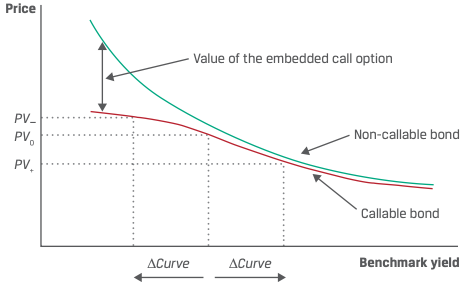
\includegraphics[scale=0.5]{/fi/callablebondrisk} \hfill
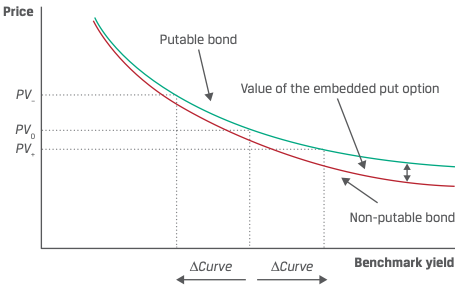
\includegraphics[scale=0.5]{/fi/putablebondrisk}
\caption{Interest rate risk characteristics of a callable bond and a putable bond}
\end{figure}

\begin{remark} \hlt{Effective Duration, Convexity Characteristics of Callable Bond}\\
Price of the non-callable bond is always greater than comparable callable bond; difference is embedded call option which is held by bond issuer.\\
When interest rates are high relative to coupon rate, value of call option is low.\\
When rates are low, the value of the call option is high since issuer is more likely to exercise the option to refinance debt at the lower prevailing rates.\\
Investor bears “call risk”. If the bond is called, investor must reinvest the proceeds at a lower interest rate.\\
When benchmark rates are high, effective duration of callable and non-callable bonds are very similar.\\
When benchmark rates are low, effective duration of callable bond is lower than comparable non-callable bond, as callable bond price does not increase as much when benchmark yields fall; call option limits price appreciation.
\end{remark}

\begin{remark} \hlt{Effective Duration, Convexity Characteristics of Putable Bond}\\
Price of putable bond is always higher than comparable non-putable bond; difference is embedded put option as held by investor.\\
Putable bond allows investor to sell bond back to issuer before maturity, usually at par value, protecting the investor from higher benchmark yields that would otherwise drive the bond’s price below par.\\
When benchmark rates are low, effective duration of putable and non-putable bonds are very similar.\\
When benchmark rates are high, put option is more valuable to investor, since the ability to sell the bond back to the issuer at par limits the price depreciation as rates rise.
\end{remark}

\begin{remark} \hlt{Computing the Effective Duration and Convexity in Practice}
\begin{enumerate}[label=\roman*.]
\setlength{\itemsep}{0pt}
\item Given price $PV_0$, compute implied OAS to the benchmark yield curve at appropriate interest rate volatility
\item Shift benchmark curve down, generate new interest rate tree, revalue bond using OAS earlier for $PV_{-}$.
\item Shift benchmark curve up, generate new interest rate tree, revalue bond using OAS earlier for $PV_{+}$.
\item Compute bond's effective duration and convenxity
\end{enumerate}
\end{remark}

\begin{remark} \hlt{Effective Durations of Callable, Putable, Straight Bonds}
\begin{enumerate}[label=\roman*.]
\setlength{\itemsep}{0pt}
\item Effective duration of callable $\leq$ Effective duration of straight
\item Effective duration of putable $\leq$ Effective duration of straight
\item Effective duration of zero-coupon $\approx$ Maturity of the bond
\item Effective duration of fixed-rate coupon bond $<$ Maturity of the bond
\item Effective duration of floater $\approx$ time (in years) to next reset
\end{enumerate}
Effective duration of straight bonds is relatively unaffected by changes in interest rates.\\
Increase in interest rates will increase effective duration of callable bond, decrease that of putable bond.
\end{remark}

\begin{figure}[H]
\centering
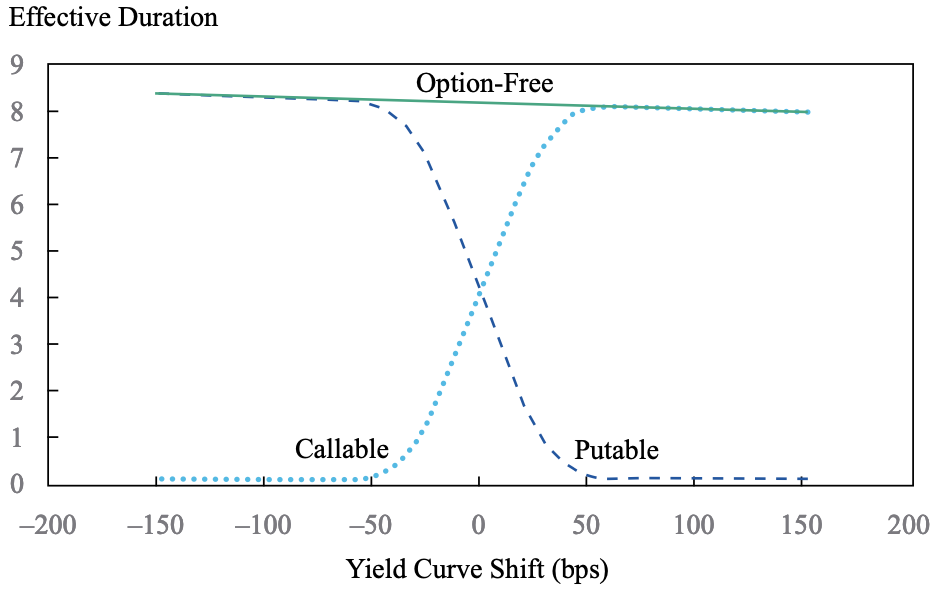
\includegraphics[scale=0.6]{/fi/effdurofoptionbonds}
\caption{Effective Durations of Option-Free, Callable and Putable Bonds}
\end{figure}

\begin{remark} \hlt{Effective Convexities of Callable, Putable, Straight Bonds}
\begin{enumerate}[label=\roman*.]
\setlength{\itemsep}{0pt}
\item Straight bonds have positive effective convexity; increase in value of option-free bond is higher when rates fall than decrease in value when rates increase by equal amount
\item Callable bonds unlikely to be called when rates are high, hence have positive convexity. When underlying call option is near its money, effective convexity turns negative; upside potential of the bond's price is limited to the call while downside is not protected
\item Putable bonds exhibit positive convexity throughout
\end{enumerate}
\end{remark}

\begin{remark} \hlt{Relation to Full Price of Bond}\\
The following relation holds in relation to the full price of the bond.
\begin{equation}
\% \Delta PV^{\text{Full}} \approx (-\text{EffDur} \times \Delta \text{Curve}) + \left[ \frac{1}{2} \times \text{EffConv} \times (\Delta \text{Curve})^2 \right] \nonumber
\end{equation}
\end{remark}

\begin{definition} \hlt{Key Rate Duration}\\
Measure of bond’s sensitivity to change in benchmark yield at a specific maturity (sensitivity to \hlt{shaping risk}).\\
Better at capturing interest rate sensitivity than simple effective duration for embedded option bonds.\\
Used to identify interest rate risk from changes in shape of the yield curve.
\begin{align}
\text{KeyRateDur}_k &= - \frac{1}{PV} \times \frac{\Delta PV}{\Delta r_k} \nonumber \\
\text{EffDur} &= \sum\limits_{k=1}^n \text{KeyRateDur}_k \nonumber \\
\frac{\Delta PV}{\Delta r_k} &= -\text{KeyRateDur}_k \times \Delta r_k \nonumber
\end{align}
where $r_k$ represents the $k$th key rate.
\end{definition}

\begin{figure}[H]
\centering
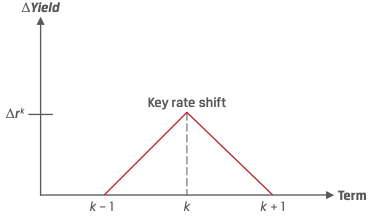
\includegraphics[scale=0.57]{/fi/keyrateshiftone}
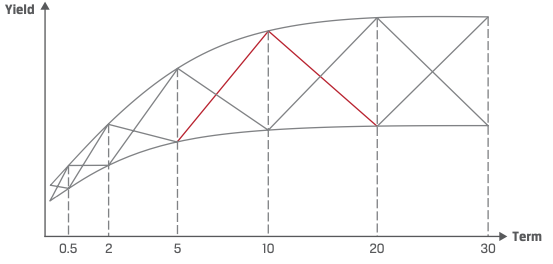
\includegraphics[scale=0.47]{/fi/keyrateshifttwo}
\caption{Key rate shift at single point, and across the benchmark curve}
\end{figure}

\begin{remark} 
\label{rem:genresultkeyratedur}
\hlt{General Results on Key Rate Duration}
\begin{enumerate}[label=\roman*.]
\setlength{\itemsep}{0pt}
\item If option-free bond is trading at par, bond's maturity-matched rate is only rate that affect bond's value. Its maturity key rate duration is same as its effective duration, and all other key rate durations are zero.
\item If option-free bond is not trading at par, the maturity-matched rate is still the most important rate.
\item Bonds with low or zero coupon may have negative key rate durations for horizons other than maturity.
\item Callable bond with low coupon is unlikely to be called; hence bond's maturity-matched rate is the most critical (i.e., highest key rate duration corresponds to bond's maturity).
\item All else equal, higher coupon bonds are more likely to be called, hence time-to-exercise rate will dominate the time-to-maturity rate.
\item Putable bonds with highest coupon rates are unlikely to be put, hence are most sensitive to maturity-matched rates.
\item All else equal, lower coupon bonds are more likely to be put, hence time-to-exercise rate will tend to dominate the time-to-maturity rate.
\end{enumerate}
\end{remark}

\begin{figure}[H]
\centering
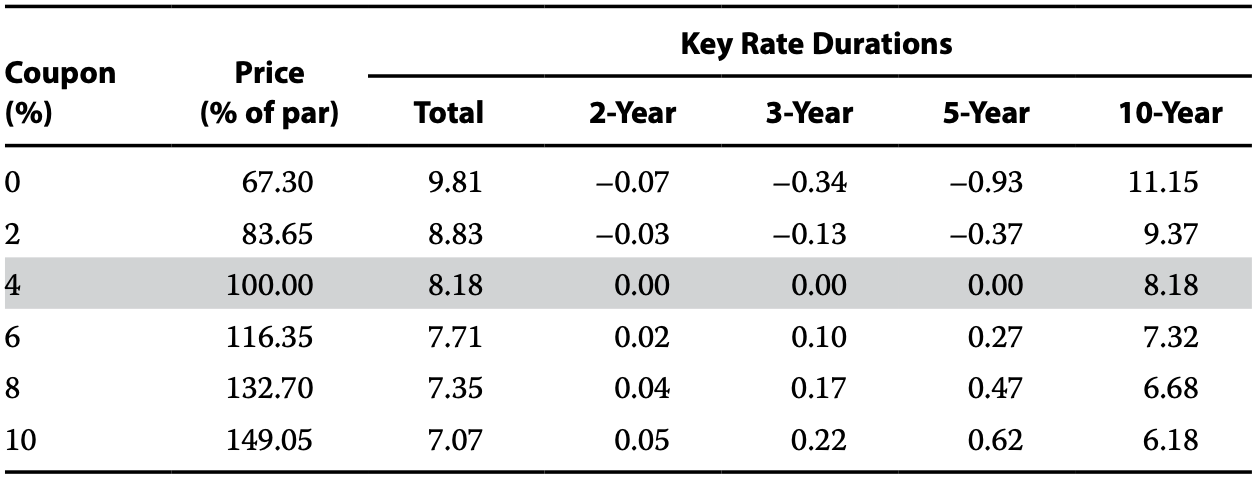
\includegraphics[scale=0.6]{/fi/keyratedurex}
\caption{Reference for Remark \ref{rem:genresultkeyratedur} (i) to (iii), KRDur for $10$-Year Option-Free Bonds at $4\%$ Flat Curve}
\end{figure}

\begin{figure}[H]
\centering
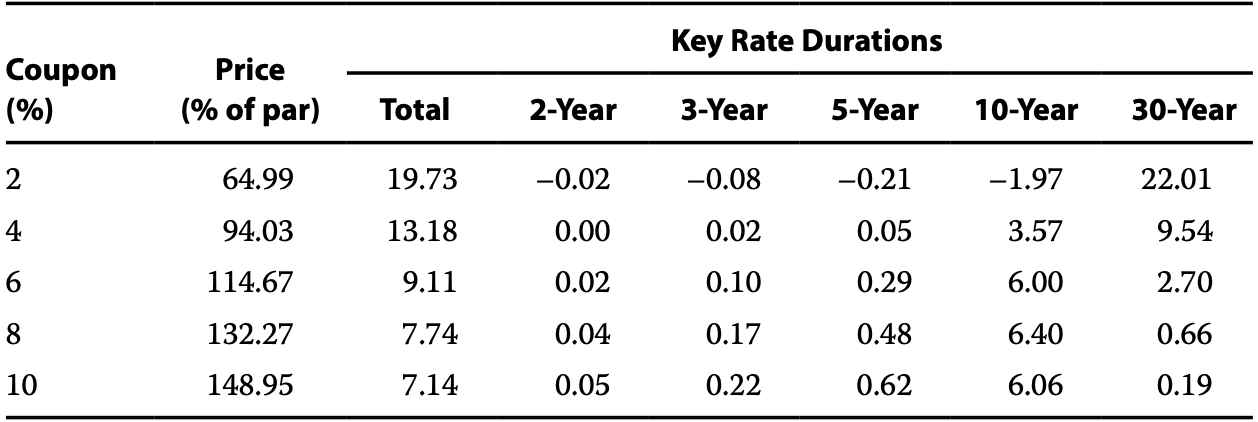
\includegraphics[scale=0.6]{/fi/keyratedurex2}
\caption{Reference for Remark \ref{rem:genresultkeyratedur} (iv) and (v), KRDur for $10$-Year Callable Bonds at $4\%$ Flat, $15\%$ Vol}
\end{figure}

\begin{figure}[H]
\centering
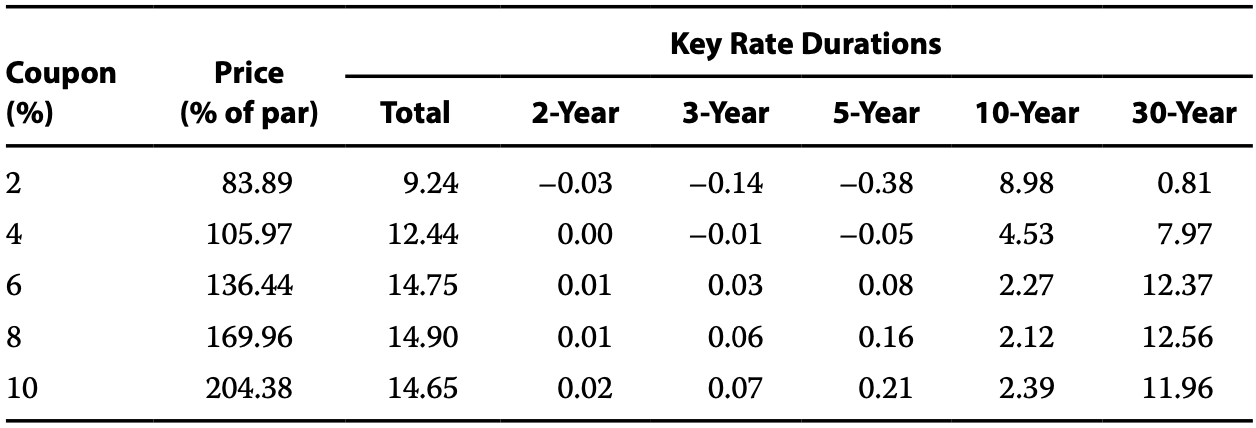
\includegraphics[scale=0.6]{/fi/keyratedurex3}
\caption{Reference for Remark \ref{rem:genresultkeyratedur} (vi) and (vii), KRDur for $10$-Year Putable Bonds at $4\%$ Flat, $15\%$ Vol}
\end{figure}

\begin{remark} \hlt{One-Sided Durations}\\
For bonds with embedded options, durations that apply only when interest rates rise/fall are better at capturing interest rate sensitivity than simple effective duration.\\
If underlying option is at-the-money, callable bonds will have lower one-sided down-duration than one-sided up-duration; price change of callable when rates fall is smaller than price change for equal increase in rates. Conversely, a near-the-money putable will have larger one-sided down-duration than one-sided up-duration.
\end{remark}

\begin{flushleft}
Summary of Curve-Based and Empirical Duration Statistics
\begin{tabularx}{\textwidth}{p{7em}|X|X}
\hline
\rowcolor{gray!30}
Measure & Definition & Interpretation \\
\hline
ApproxModDur & Estimates slope of line tangent to bond’s price–yield curve & Yield-based method to estimate ModDur \\
\hline
EffDur & Sensitivity of a bond’s price to a change in a benchmark yield curve & Curve-based method to estimate ModDur for complex bonds with uncertain cash flows \\
\hline
Key Rate & Measures bond sensitivity to benchmark yield change for a specific maturity & Partial duration statistic that gauges bond’s sensitivity to non-parallel benchmark yield curve changes \\
\hline
Empirical & Measure using historical data in statistical models and incorporating factors affecting bond prices to determine the price–yield relationship & Statistical estimate that accounts for correlation between yield spreads and benchmark yield-to-maturity changes under different economic scenarios \\
\hline
\end{tabularx}
\end{flushleft}